\section{Тор}
\textbf{Вопрос.} Что такое тор, по которому усредняется $\delta$?

После нормальной формы остаются три амплитуды и три фазы. Тор --- все тройки фаз при фиксированных амплитудах. Это не траектория: один оборот ставит на тор одну точку, долгий трекинг наматывает нитку. $\delta_{\mathrm{eq}}$ --- среднее $\delta$ по всей поверхности сразу.

\begin{figure}[H]\centering
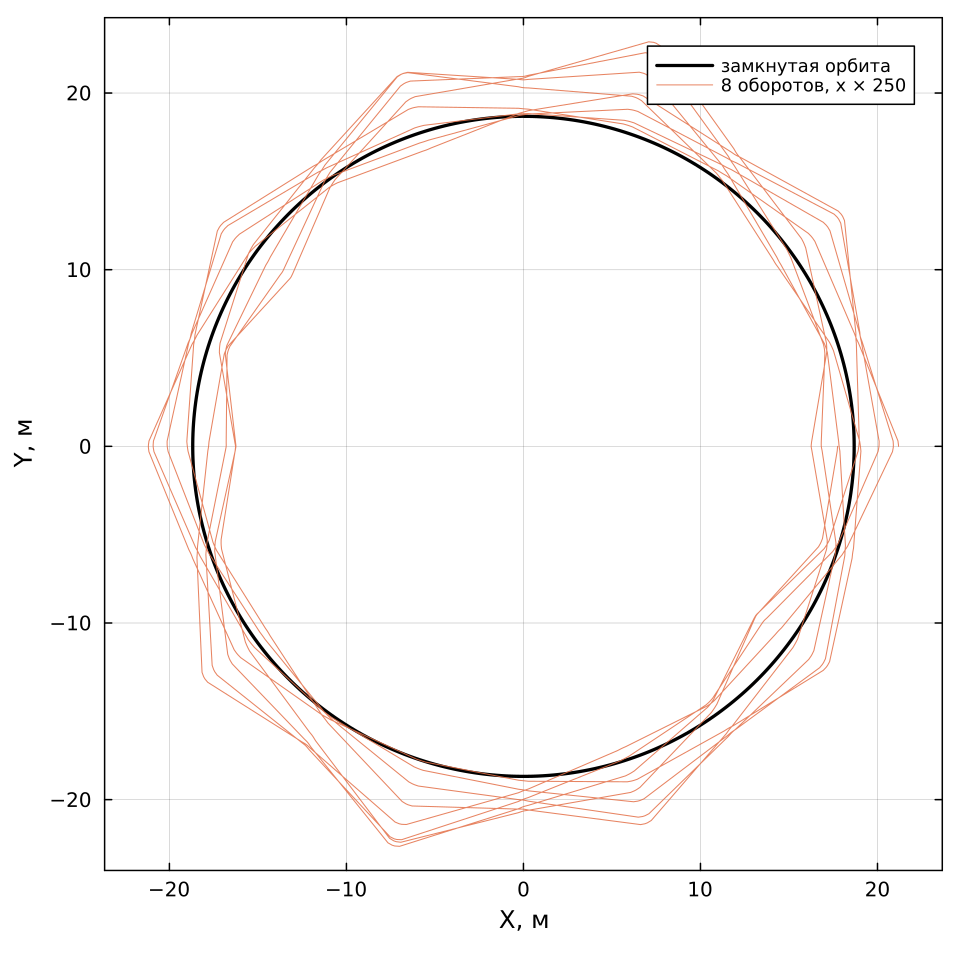
\includegraphics[width=0.72\textwidth]{figs/fig_08_torus_ring.png}
\caption{План кольца, 8 оборотов. Поперечник увеличен в $\vtorScale$ раз. Полоса, которую заполняет траектория, --- тор вокруг машины.}
\end{figure}

\begin{figure}[H]\centering
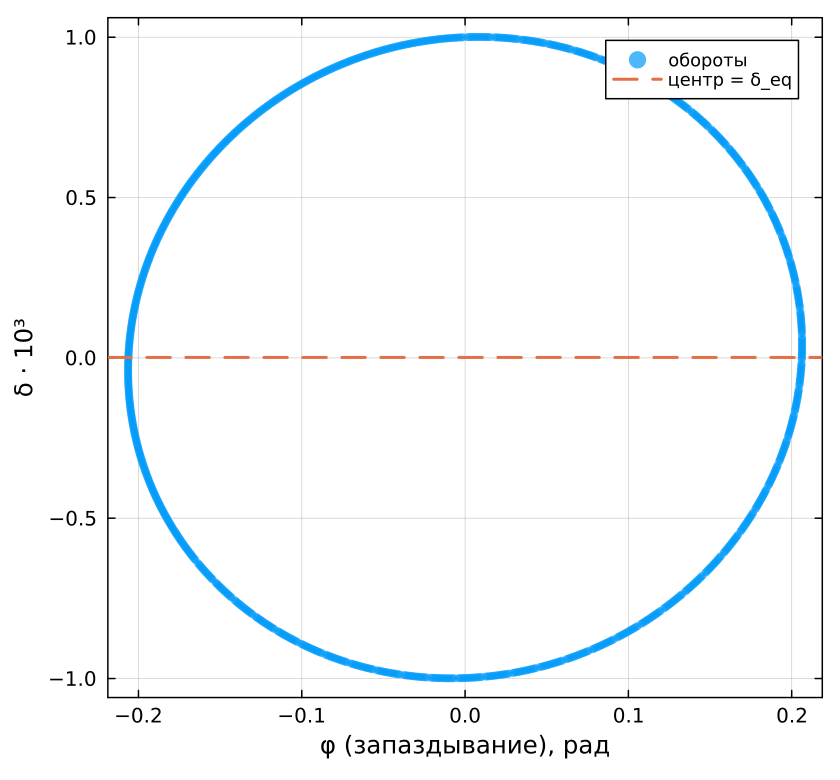
\includegraphics[width=0.62\textwidth]{figs/fig_08_synchrotron.png}
\caption{Плоскость $(\varphi,\delta)$ при включённом ВЧ. Частица ходит по окружности. Центр --- $\delta_{\mathrm{eq}}=\vdeqTorus$; в центр частица не садится.}
\end{figure}

\begin{figure}[H]\centering
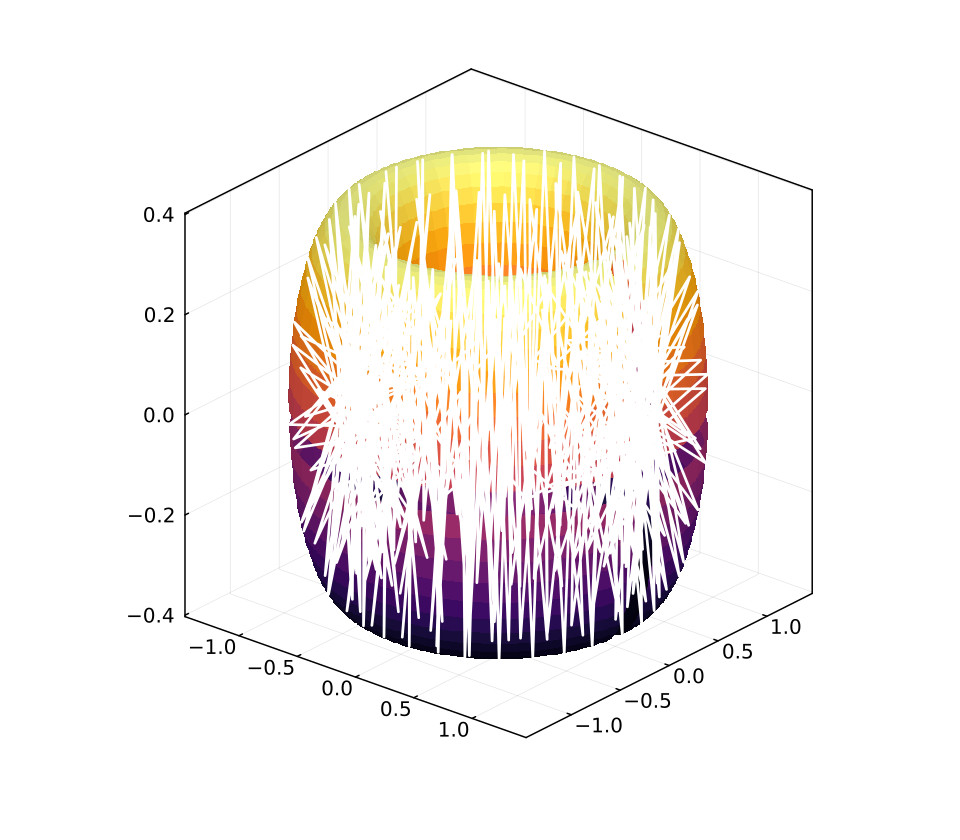
\includegraphics[width=0.72\textwidth]{figs/fig_08_torus_surface.png}
\caption{Поверхность $(\theta_\beta,\theta_s)$ при $J_y=0$. Цвет --- лабораторный $\delta$. Среднее цвета $\vmeanColor$, M2 $\vmtwoTorus$. Белая нитка --- точный интегратор. Полный тор трёхмерен: вторая бетатронная фаза на этом срезе не показана.}
\end{figure}

\textbf{Вывод.} $\delta_{\mathrm{eq}}$ --- среднее по поверхности, не точка, в которую частица приходит. Трекинг рисует одну нитку на этом торе.
